%
%  $Author: ienne $
%  $Date: 1995/09/15 15:20:59 $
%  $Revision: 1.4 $
%

% \documentclass[10pt,journal,cspaper,compsoc]{IEEEtran}   %%%tc version
\documentclass[10pt, conference]{IEEEtran}
%\documentclass[conference,compsoc]{IEEEtran}
%\documentclass[10pt, conference]{IEEEtran}
%\documentclass[times, 10pt,onecolumn]{article}
\usepackage{amsmath, amssymb, enumerate}
\usepackage{semantic}
\usepackage{soul}
\usepackage{listings}

%%%%%%%%%%%%%%%% page control%%%%%%%%%%%%%%%%%
%\usepackage[margin=0.75in]{geometry}

%\linespread{0.991}  %%%%%%%%%%%%%%%%%%%%%%%%%%%%%%%%% this is really useful
%\usepackage{cite}
\usepackage{fancybox}
\usepackage{amsfonts}
%\usepackage{algorithm}
%\usepackage[noend]{algorithmic}
\usepackage[usenames]{color}
%\usepackage{colortbl}
%\usepackage[ figure, boxed, vlined]{algorithm2e}
%\usepackage[linesnumbered,vlined]{algorithm2e}
%\usepackage[lined,boxed]{algorithm2e}
\usepackage{listings}

\usepackage[linesnumbered,vlined]{algorithm2e}
\usepackage{graphicx}
\usepackage{times}
\usepackage{psfrag}
\usepackage{subfigure}
\usepackage{caption}
%\usepackage{subcaption}
\usepackage{multirow}
%\usepackage{setspace}
%\usepackage{listings}
\usepackage{epsfig}
%\usepackage{epstopdf}
%\usepackage[font=small,labelfont=bf]{caption}
% \usepackage{url}
\usepackage[hyphens]{url}

\usepackage{color}
\def\fixme#1{\typeout{FIXED in page \thepage : {#1}}
%\bgroup \color{red}{} \egroup}
\bgroup \color{red}{[FIXME: {#1}]} \egroup}

\lstset{breaklines=true, basicstyle=\ttfamily\fontsize{6}{7}\selectfont, escapeinside={(*@}{@*)}}

%\usepackage[pdftex]{hyperref}
\usepackage{rotating,tabularx}

\interfootnotelinepenalty=10000

%% Define a new 'leo' style for the package that will use a smaller font.
\makeatletter
\def\url@leostyle{%
  \@ifundefined{selectfont}{\def\UrlFont{\sf}}{\def\UrlFont{\small\ttfamily}}}
\makeatother

%\documentstyle[times,art10,twocolumn,latex8]{article}

%-------------------------------------------------------------------------
% take the % away on next line to produce the final camera-ready version
\pagestyle{plain}
%\thispagestyle{empty}
%\pagestyle{empty}

\newtheorem{theorem}{Theorem}
\newtheorem{lemma}[theorem]{Lemma}


%% remaining budget share, used in task stall section.
\newcommand{\bottomrule}{\hline}
\newcommand{\toprule}{\hline}
\newcommand{\midrule}{\hline}

\setlength\extrarowheight{1.5pt}
\setlength{\tabcolsep}{1pt}

\newcommand{\ttt}{\texttt}
\newcommand{\rarr}{\rightarrow}
\newcommand{\sarr}{\leadsto}

%-------------------------------------------------------------------------
\begin{document}

\title{A Domain Specific Language for SpectreGuard}
\author{David Young\\
d063y800@ku.edu\\
University of Kansas, USA\\
}

\maketitle
\thispagestyle{empty}
\begin{abstract}

  A Spectre mitigation strategy in the form of a mechanism for marking variables
  as ``non-speculative'' was developed in \cite{SpectreGuard}. In this paper, we
  develop an embedded domain specific language (EDSL) in Haskell to provide
  support for this feature, with a backend that generates C code. The static
  type system of Haskell is used so that many basic forms of copying secret
  variables to public variables are disallowed. Additionally, a static analysis
  was developed which will detect some cases of secret variables leaking to
  public variables via control flow constructs.

\end{abstract}

%-------------------------------------------------------------------------

\section{Introduction}
\label{sec:Introduction}
SpectreGuard is provides an abstraction that allows programmers to prevent
speculative access of certain variables.~\cite{SpectreGuard} As Spectre-based
attacks remain an issue, even in modern computer systems, such mitigations and
preventative measures are crucial to maintaining the security of software.  For
preserving program correctness, static analyses are desirable to prevent
programmers from accidentally successfully compiling code which copies a
``secret'' variable (a variable protected by SpectreGuard) to a ``public''
variable (a variable with no such protection). To this end, two interrelated
static analysis techniques are designed and implemented.

In this paper, we make the following contributions:

\begin{itemize}
\item We describe a small domain specific language embedded in Haskell for representing
  simple C programs (Section~\ref{sec:Syntax}).
\item A code generator which generates C code from this EDSL is outlined
  (Section~\ref{sec:Syntax}).
\item We give a system of types which causes the expression language of this
  EDSL to be statically checked for variable copies that directly leak memory
  from secret variables to public variables (Section~\ref{sec:SensTypes}).
\item Another static analysis procedure is given which can find \textit{indirect}
  leak paths through control structures (Section~\ref{sec:Analysis}). This analysis
  procedure can be applied to EDSL code in the same way as the code generator
  can be applied to EDSL code. The results from this analysis take the form
  of a forest of multiway trees, providing information about these possible
  indirect leaks.
\item We provide several examples and describe how the system handles them
  (Section~\ref{sec:Examples}).
\end{itemize}

\section{Background}

Haskell is a purely functional programming language with strong static type
system based on System F and algebraic datatypes (ADTs).~\cite{HistoryOfHaskell}
These features, particularly the type system, the algebraic datatypes and its
support for higher-order functions, make it a powerful tool for the creation of
EDSLs. Expressions, commands and programs (compound commands) can be
straightforwardly expressed using ADTs using a \textit{deep
embedding}.~\cite{DeepAndShallow}

A deep embedding directly exposes its abstract syntax tree (AST) as a value.
This allows EDSL programs to be easily manipulated and examined, such as for
interpretation, code generation and static analysis (the latter two we make use
of in this paper).

\section{Syntax}
\label{sec:Syntax}
A correspondence between the syntax of the EDSL, which is inherited from
Haskell, and the C language is given in Fig. \ref{fig:Syntax}. In the right column, an
overline indicates that the transformation from EDSL to C is recursively
performed to the expression or command underneath the overline.

This also outlines procedure that the C code generator uses. When code written
in the EDSL is transformed into C code, a name generator first annotates the
abstract syntax tree (AST) with globally unique names (enforcing the Barendregt
variable convention; see Chapter 2 in~\cite{BarendregtConversion}). This
annotated AST can be used by both the code generator and the information flow
leak analysis tool (the latter is described in Section \ref{sec:Analysis}). The
code generator performs a transformation from code in the syntax given in the
left column of Fig.~\ref{fig:Syntax} to the right column of the figure. This is
transformation recursively applies itself when it reaches the parts marked with
an overline in the right column of the figure. It is worth noting that, as a
result of this technique, the names in the generated C code will not generally
be the same as the names in the EDSL code.

The one major aspect of the C code generator that is not described in this table
is how the loop variable in \ttt{for} loops can be tagged as secret (if appropriate).
This is accomplished by recovering the type-level sensitivity type information at
runtime. Such a recovery is made possible by the use of singletons.~\cite{Singletons}
\ttt{for} loops provide a particular example of where Haskell's support for higher-order function
can be used inside an EDSL to implement commands that involve the creation of
new variables.

Code can be written in this EDSL by importing the EDSL's package in standard
Haskell code and using the Glasgow Haskell Compiler (GHC) to compile the code.
Note that as a result of this design, all standard Haskell programming language
constructs are available for metaprogramming purposes.  Examples written in this
EDSL syntax are given in Section \ref{sec:Examples}.

\begin{figure}
\begin{tabular}{|l|l|}
  \hline
  EDSL syntax & C syntax \\
  \hline
  \begin{lstlisting}
  v <- decl x
  \end{lstlisting}
  & \begin{lstlisting}[language=C]
  int v = x;
  \end{lstlisting}\\

  \hline
  \begin{lstlisting}
  v <- allocPublic @Int n
  \end{lstlisting}
  & \begin{lstlisting}[language=C]
  int v[n];
  \end{lstlisting}\\

  \hline
  \begin{lstlisting}
  v <- allocPrivate @Int n
  \end{lstlisting}
  & \begin{lstlisting}[language=C]
  int v[n] __attribute__((__nospec__));
  \end{lstlisting}\\

  \hline
  \begin{lstlisting}
  arrA .= arrB
  \end{lstlisting}
  & \begin{lstlisting}[language=C]
  memcpy(arrA, arrB, sizeof(arrA));
  \end{lstlisting}\\

  \hline
  \begin{lstlisting}
  i .= j
  \end{lstlisting}
  & \begin{lstlisting}[language=C]
  i = j;
  \end{lstlisting}\\

  \hline
  \begin{lstlisting}
  arr ! i
  \end{lstlisting}
  & \begin{lstlisting}[language=C]
  arr[i]
  \end{lstlisting}\\

  \hline
  \begin{lstlisting}
  x <? y
  \end{lstlisting}
  & \begin{lstlisting}[language=C]
  x < y
  \end{lstlisting}\\

  \hline
  \begin{lstlisting}
  while cond body
  \end{lstlisting}
  & \begin{lstlisting}[language=C]
  while ((*@$\overline{\ttt{cond}}$@*)) { (*@$\overline{\ttt{body}}$@*) }
  \end{lstlisting}\\

  \hline
  \begin{lstlisting}
  ifThenElse cond t f
  \end{lstlisting}
  & \begin{lstlisting}[language=C]
  if ((*@$\overline{\ttt{cond}}$@*)) { (*@$\overline{\ttt{t}}$@*) } else { (*@$\overline{\ttt{f}}$@*) }
  \end{lstlisting}\\

  \hline
  \begin{lstlisting}
  for init
    (\i ->
      (cond, update, body))
  \end{lstlisting}
  & \begin{lstlisting}[language=C]
  for (int i = (*@$\overline{\ttt{init}}$@*); (*@$\overline{\ttt{cond}}$@*); (*@$\overline{\ttt{update}}$@*))
    { (*@$\overline{\ttt{body}}$@*) }
  \end{lstlisting}\\


  \hline
\end{tabular}
\caption{Syntax of the EDSL vs C syntax}
\label{fig:Syntax}
\end{figure}

\section{Sensitivity Types}
\label{sec:SensTypes}
The Haskell type system is leveraged to perform a basic static consistency check
of the sensitivities of variables, so that a variable does not get assigned to a
variable of a different sensitivity. This is done by making the \verb|Expr| type
constructor take a phantom type argument~\cite{Phantom}. The phantom type
argument is the \textit{sensitivity type} of that expression.  The logical
inference rules corresponding to this check are given in Fig.
\ref{fig:SensTypes}. Note that the EDSL inherits the rest of Haskell's type
system in addition to these rules. Only the aspects of the type system that is
particularly relevant to the EDSL is reflected in the figure, often specialized
to the particular scenario encountered in using sensitivity types in the EDSL.
An introduction to this style of inference rule system, with many examples and
applications in the study of programming languages, is given in
\cite{HarperFoundations}.

Observe that an two expressions with different sensitivity types cannot be
combined into a larger compound expression. However, commands (represented by
the \verb|Cmd| type constructor) often have expressions embedded in them and
commands can be sequenced with each other.  There is no restriction on how two
commands can be combined, even if they involve expressions with different
sensitivity types. This freedom in combining commands independently of
sensitivity foreshadows the essence of the problem we will encounter in
Section \ref{sec:Analysis}. For now, note that all control flow constructs are
part of the command type (as opposed to the expression type).

Singletons~\cite{Singletons} are used to preserve this type level at runtime, so that the
code generator can generate SpectreGuard annotations where appropriate. These annotations can
then be used by the SpectreGuard mitigation system.~\cite{SpectreGuard}

In Fig. \ref{fig:SensTypes}, it is assumed that $\tau$ and $\sigma$ are given by the
following grammar:
\begin{gather*}
  \sigma ::= \ttt{Public}\;|\;\ttt{Secret}\\
  \tau ::= \ttt{Int}\;|\;\ttt{Ptr}\;\tau\\
  \alpha ::= \ttt{()}\;|\;\ttt{Expr $\sigma$ $\tau$}
\end{gather*}

\noindent A typing judgement is expressed with the syntax

\begin{equation*}
  \ttt{x :: $\beta$}
\end{equation*}

\noindent where \ttt{x} is some expression or command in the EDSL. This judgement means
that \ttt{x} has type $\beta$. This is also the same syntax used by Haskell, and by extension
the EDSL, to explicitly specify the type of any expression when necessary or desired.


\begin{figure}
  \centering
\resizebox{0.67\linewidth}{!}{
\begin{minipage}{\linewidth}
  \centering
  \openup 3mm
\begin{gather*}
  \inference{}{\ttt{Public :: Sensitivity}}\\
  \inference{}{\ttt{Secret :: Sensitivity}}\\
  \inference{n \in \mathbb{N}}{\ttt{$n$ :: Int}}\\
  \inference{n \in \mathbb{N}}{\ttt{$n$ :: Expr $\sigma$ Int}}\\
  \inference{%
    \Gamma \vdash \ttt{x :: Expr $\sigma$ Int}
    & \Gamma \vdash \ttt{y :: Expr $\sigma$ Int}}
    {\Gamma \vdash \ttt{x + y :: Expr $\sigma$ Int}}\\
  \inference{%
    \Gamma \vdash \ttt{x :: Expr $\sigma$ Int}
    & \Gamma \vdash \ttt{y :: Expr $\sigma$ Int}}
    {\Gamma \vdash \ttt{x <? y :: Expr $\sigma$ Bool}}\\
  \inference{%
    \Gamma \vdash \ttt{a :: Expr $\sigma$ (Ptr $\tau$)}
    & \Gamma \vdash \ttt{i :: Expr $\sigma$ Int}}
    {\Gamma \vdash \ttt{a ! i :: Expr $\sigma$ $\tau$}}\\
  \inference{\Gamma \vdash \ttt{n :: Int}}{\Gamma \vdash \ttt{allocPublic @$\tau$ n :: Cmd (Expr Public (Ptr $\tau$))}}\\
  \inference{\Gamma \vdash \ttt{n :: Int}}{\Gamma \vdash \ttt{allocSecret @$\tau$ n :: Cmd (Expr Secret (Ptr $\tau$))}}\\
  \inference{\Gamma \vdash \ttt{x :: $\tau$}}{\Gamma \vdash \ttt{decl x :: Cmd (Expr Public $\tau$)}}\\
  \inference{%
    \Gamma \vdash \ttt{x :: Expr $\sigma$ $\tau$}
    & \Gamma \vdash \ttt{y :: Expr $\sigma$ $\tau$}}
    {\Gamma \vdash \ttt{x .= y :: Cmd ()}}\\
  \inference{%
    \Gamma \vdash \ttt{cond :: Expr $\sigma$ Bool}
    \\ \Gamma \vdash \ttt{t :: Cmd $\alpha$}
    &\Gamma \vdash \ttt{f :: Cmd $\alpha$}}
    {\Gamma \vdash \ttt{ifThenElse cond t f :: Cmd ()}}\\
  \inference{%
    \Gamma \vdash \ttt{cond :: Expr $\sigma$ Bool}
    & \Gamma \vdash \ttt{body :: Cmd $\alpha$}}
    {\Gamma \vdash \ttt{while cond body :: Cmd ()}}\\
  \inference{%
    \Gamma \vdash \ttt{init :: Expr $\sigma$ $\tau$}\\
    \Gamma \vdash \ttt{fn :: Expr $\sigma$ $\tau$ $\rarr$ (Expr $\sigma$ Bool, Cmd (), Cmd ())}
    }{\Gamma \vdash \ttt{for init fn :: Cmd ()}}\\
  \inference{%
    \Gamma \vdash \ttt{c :: Cmd (Expr $\sigma$ $\tau$)}
    \\ \Gamma,\ttt{(x :: Expr $\sigma$ $\tau$)} \vdash \ttt{rest :: Cmd $\alpha$}
  }{%
    \Gamma \vdash \ttt{(\textbf{do} \{ x <- c; rest \}) :: Cmd $\alpha$}
  }\\
  \inference{%
    \Gamma \vdash \ttt{c :: Cmd (Expr $\sigma$ $\tau$)}
    \\ \Gamma \vdash \ttt{rest :: Cmd $\alpha$}
  }{%
    \Gamma \vdash \ttt{(\textbf{do} \{ c; rest \}) :: Cmd $\alpha$}
  }
\end{gather*}
\end{minipage}}
  \caption{Typing rules for sensitivity types}
\label{fig:SensTypes}
\end{figure}

\section{Examples}
\label{sec:Examples}

A couple of simple examples illustrate the basic typing rules:

\begin{lstlisting}[language=haskell]
example1 :: Cmd ()
example1 = do
  array1 <- allocSecret @Int 8
  array2 <- allocSecret @Int 8
  array2 .= array1
\end{lstlisting}

\noindent This first example passes the type checker with no problem: the array copy
is being performed from one secret array to another secret array.

The next example does not type check:

\begin{lstlisting}[language=haskell]
  -- This example fails to type check
example2 :: Cmd ()
example2 = do
  array1 <- allocSecret @Int 8
  array2 <- allocPublic @Int 8
  (*@\color{red}array2 .= array1@*)
\end{lstlisting}

\noindent \ttt{example2} fails to type check since \ttt{array1} and \ttt{array2} have
different sensitivity annotations, while the type of the \ttt{(.=)} operation
requires that both arguments have the same sensitivity annotation. This restriction can
be seen in the typing rule for \ttt{(.=)} in Fig. \ref{fig:SensTypes}.

Turning to more complex examples, we can see that the following example type checks

\begin{lstlisting}[language=Haskell]
example3 :: Cmd ()
example3 = do
  arrayA <- allocSecret @Int 8
  arrayB <- allocSecret @Int 8
  for (0 :: Expr Secret Int) (\i -> ((i <? 8), (i += 1), do
    (arrayA ! i) .= (arrayB ! i)))
\end{lstlisting}

\noindent This demonstrates a basic \ttt{for} loop and the array indexing syntax. Again, the
only copies happen between two variables with the same sensitivity level, so this
program is well-typed.

The next slightly more complex example exhibits an important limitation of this sensitivity type checking:

\begin{lstlisting}[language=Haskell]
example4 :: Cmd ()
example4 = do
  secretArray <- allocSecret @Int 8
  publicArray <- allocPublic @Int 8

  for (0 :: Expr Public Int) (\i -> ((i <? 8), (i += 1), do
    leak <- decl (0 :: Int)
    for (0 :: Expr Secret Int) (\j -> ((j <? (secretArray ! i))
                                      ,(j += 1), do
      leak += 1))
    (publicArray ! i) .= leak))
\end{lstlisting}

\noindent Even though this code type checks without error, the entire contents of the secret variable \ttt{secretArray} is leaked
to the public variable \ttt{publicArray}. The leak occurs despite the fact that the two variables have different
sensitivity annotations. This is the
result of information being indirectly leaked from the secret variable to the
public variable via a control flow construct: in this case, the innermost \ttt{for} loop. Such an example has been studied from programming language perspective before; for instance
in~\cite{InfoFlowAnalysis}.

This kind of leak directly motivates the analysis in Section \ref{sec:Analysis}. This analysis will perform
some level of checking beyond the relatively basic sensitivity type check described so far.

\section{Information Flow Analysis}
\label{sec:Analysis}

In Section \ref{sec:Examples}, a significant limitation of the sensitivity type checking
was outlined. In this section we address this limitation using a static analysis technique.
Possible leaks from secret variables to public variables via control flow constructs will
be analyzed and the results of this analysis will be described in the form of
a forest of trees, given in DOT format (which can then be converted to other formats,
such as PDF)~\cite{DOT}. The C code generated from \ttt{example4} is shown in Fig. \ref{fig:GenC4}.
Note that the secret array is named \verb|_fs_0| and the public array is named \verb|_fs_1| by the
code generator. From the original \ttt{example4}, the information flow analyzer generates the
graph given in Fig. \ref{fig:Analysis4}. Secret variables are represented as nodes with
a rectangular shape and public variables are represented as nodes with an elliptic shape. An
arrow going from one node to another represents a possible information leak from the first
node to the second node due to a control flow construct.

\begin{figure}
\begin{center}
\begin{tabular}{c}
\begin{lstlisting}{language=C}
int _fs_0[8] __attribute__((nospec))__;
int _fs_1[8];
for (int _fs_2 = 0; _fs_2 < 8; _fs_2 = _fs_2 + 1)
{
  int _fs_3 = 0;
  for (int _fs_4 __attribute__((nospec))__ = 0;
      fs_4 < (_fs_0[_fs_2]);
      _fs_4 = _fs_4 + 1)
  {
    _fs_3 = _fs_3 + 1;
  }
  _fs_1[_fs_2] = _fs_3;
}
\end{lstlisting}
\end{tabular}
\end{center}
\caption{C code generated from \ttt{example4}}
\label{fig:GenC4}
\end{figure}

\begin{figure}
\centering
  \resizebox{0.3\columnwidth}{4cm}{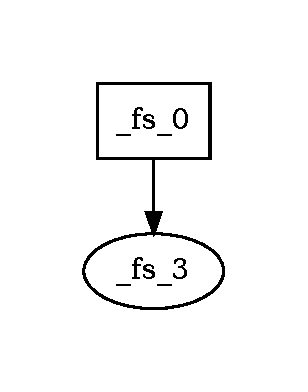
\includegraphics{Diagrams/example4-analysis.pdf}}
\caption{Results of leak analysis on \ttt{example4}}
\label{fig:Analysis4}
\end{figure}

A more complicated example is \ttt{example5} in the following:

\begin{lstlisting}[language=Haskell]
example5 :: Cmd ()
example5 = do
  secretArray <- allocSecret @Int 8
  publicArray <- allocPublic @Int 8
  for (0 :: Expr Public Int) (\i -> ((i <? 8), (i += 1), do
    leak <- decl (0 :: Int)
    for (0 :: Expr Secret Int) (\j -> ((j <? (secretArray ! i))
                                      ,(j += 1), do
      leak += 1))
    (publicArray ! i) .= leak))
  secretArrayA <- allocSecret @Int 8
  secretArrayB <- allocSecret @Int 8
  publicArray2 <- allocPublic @Int 8
  secretArrayA .= secretArray
  secretArrayB .= secretArrayA
  for (0 :: Expr Public Int) (\i -> ((i <? 8), (i += 1), do
    leak2 <- decl (0 :: Int)
    for (0 :: Expr Secret Int) (\j -> ((j <? (secretArrayB ! i))
                                      ,(j += 1), do
      leak2 += 1)
    (publicArray2 ! i) .= leak2))
\end{lstlisting}

In the generated code for \ttt{example5}, we have the correspondence between variables in the EDSL code and the
generated C code given in the table in TABLE \ref{table:Names5}. As both the C code generator and the
static analysis tool use the same name generator, these names stay stable across the results of both. The analysis of \ttt{example5} is given in Fig. \ref{fig:Analysis5}.

The tree in resulting from the analysis shows that \ttt{secretArray} leaks to \ttt{leak}. Also, \ttt{secretArray} flows to
to \ttt{secretArrayA}, which flows to \ttt{secretArrayB}. Finally, \ttt{secretArrayB} leaks to \ttt{leak2}. Once
the analysis generates these trees, only the branches which ultimately end in a leak to a public variable
are kept. Branches which never lead to a public variable are thrown out. Also, information flow from one
public variable to another public variable is not represented. This choice was made to limit the size
of the output and prevent it from being too overwhelming to the programmer.

\begin{table}
  \centering
  \begin{tabular}{|c|c|}
    \hline
    EDSL name in \ttt{example5} & Generated C Name \\
    \hline
    \verb|secretArray| & \verb|_fs_0|\\
    \hline
    \verb|publicArray| & \verb|_fs_1|\\
    \hline
    \verb|leak| & \verb|_fs_3|\\
    \hline
    \verb|secretArrayA| & \verb|_fs_5|\\
    \hline
    \verb|secretArrayB| & \verb|_fs_6|\\
    \hline
    \verb|publicArray2| & \verb|_fs_7|\\
    \hline
    \verb|leak2| & \verb|_fs_9|\\
    \hline
  \end{tabular}
\caption{Correspondence between EDSL names and generated C names for \ttt{example5}}
\label{table:Names5}
\end{table}

\begin{figure}
\centering
  \resizebox{0.3\columnwidth}{4cm}{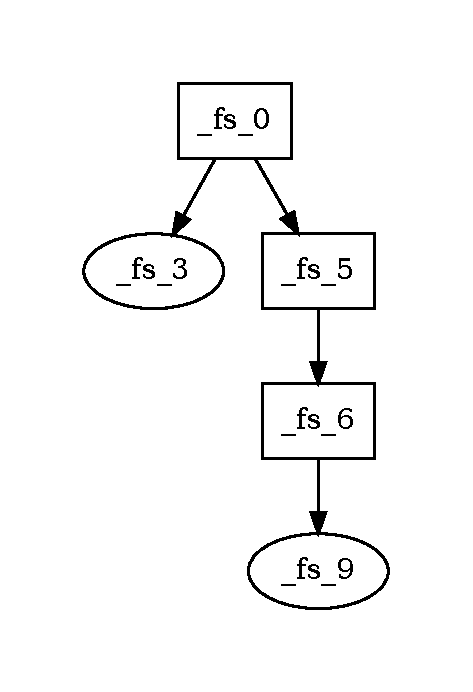
\includegraphics{Diagrams/example5-analysis.pdf}}
\caption{Results of leak analysis on \ttt{example5}}
\label{fig:Analysis5}
\end{figure}

The implementation of the analysis tool is built around two primary data
structures:

\begin{itemize}
  \item
    A forest of multi-way trees (these are also called ``rose
trees''~\cite{LooplessBird}) which represents the leak paths
  \item
    A stack of name associations (a ``scope stack''). Each entry in the stack is
    a pair consisting of two lists of names. The first list contains all of the
    names that are in the current scope: the ``in-scope list''. When a
    conditional construct is entered, all of the secret variables in the
    conditional will be put into the second list and a new pair of empty lists
    will be pushed onto the stack. This second list is the ``secret list''
\end{itemize}

When a declaration is encountered, this name is added to the current ``scope
frame'' in the scope stack. Whenever an assignment is encountered, all of the
names in the left-hand side which are contained in the in-scope list of any
scope frame \textit{before} the current one are added as children (in the rose
tree forest) of all of nodes corresponding to the names in the secret list of
the stack frame in which the left-hand side name occured.

An alternate way to view the scope stack is as a stack of \textit{relations} on
on names. Each item of the stack is a relation such that two names are related
if and only if the left-hand name is a public variable declared in the corresponding
scope and the right-hand name is a secret variable in a conditional within the scope.

This allows us to look for leaks that happen ``through'' a control construct.

The operations on the scope stack data structure have the following type signatures:

\begin{lstlisting}
emptyScope :: Scope

scopeAddName :: Scope -> Name -> Scope
scopePush :: Scope -> [Name] -> Scope
scopePop :: Scope -> Scope
publicNonLocals :: Scope -> Name -> Maybe [Name]
\end{lstlisting}

\noindent These operations are used by the tool in its analysis of an EDSL
program as follows:

Whenever a declaration is encountered in EDSL code, the corresponding variable
name is added to the scope stack with \ttt{scopeAddName}. Whenever a control
structure is entered (such as a \ttt{for} loop or an \ttt{if} statement),
\ttt{scopePush} is called with a list of all secret variables (if any) in the
condition of that control structure. When an assignment is encountered, it
uses \ttt{publicNonLocals} to see if there are any secret variables associated
to an enclosing control structure, outside of which the given name has been declared.

At the end of the algorithm, only leaves corresponding to public names are
retained. This is due to the fact that the only time a leak occurs, from the
perspective of this static analysis tool, is if a secret variable eventually
gets indirectly copied to a public variable.


\section{Related Work}
\label{sec:RelatedWork}

The way that the type-level tagging mechanism works is similar to several other
prior works. One such work is McBride's \textit{Kleisli Arrows of Outrageous
Fortune}~\cite{KleisliArrows}. In that paper, an invalid state is unable to be
reached as the result of a similar type-level tag as the \ttt{Sensitivity} tag
in the present paper: the McBride paper uses a type-level tag which indicates
whether a file handle is open or closed. However, significantly more machinery
is involved in the McBride paper, as it is necessary to put such a tag on a
monadic type. While a monadic type is used in the present paper (in the form of
the \ttt{Cmd} type), this type does not use a type-level tag. The creation of
such machinery is the main purpose of the McBride paper.

As mentioned previously, a theory of \textit{information flow} in the context of
both computer security and programming language theory has been developed. A description
of this theory is given in~\cite{InfoFlowAnalysis}.

A significant recent work also related to the use of domain specific languages
with strong, static type systems to control information flow for security
purposes is \textit{Liquid Information Flow Control} by Polikarpova et
al.~\cite{Lifty} As its title suggests, this paper also builds on the theory of information flow. In that work, a novel domain specific programming language is
developed which has a static type system that is geared specifically towards
expressing security policies at a type level. As this is done within a static
type system, these invariants are machine-verified at compile-time.  Not only
can these policy violations be detected, the system they develop is also able to
fix leaks.

More broadly, an example of a language being represented similarly, as an
pure expression language separated from a command language, can be found in
Winskel's 1993 book in the form of the \textbf{IMP} language.~\cite{WinskelBook} This
book provides an in-depth look at the three major mathematical formalizations
of programming language semantics (axiomatic semantics, operational semantics and
denotational semantics) and uses them to analyze \textbf{IMP}.


\section{Future Work}
\label{sec:FutureWork}
A further investigation into the tradeoffs and possible additional features of
the information flow analysis is likely to be useful. This could provide a more
accurate and succinct picture to programmers of where leaks are occurring, or
potentially occurring. It is possible that some of these other leak conditions
could be incorporated into the type system, by exploiting the dependent type
features enabled by singletons~\cite{Singletons} and, in the future, by
Dependent Haskell.~\cite{DepHaskSpec} Dependent types provide a powerful
technique for writing programs at a type-level, which will be executed at
compile-time by the type checker.~\cite{CertProg, DepHaskSpec} A more
lightweight technique, which might be able to be applied to allow for more
expressive policies to control of information flow within the type system, would
be the ``ghosts of departed proofs'' design technique.~\cite{DepartedProofs}

Another possible, related, future development would be the to attempt to add a
mechanism which automatically fixes some (or all) leaks. Such a system has precendent
in the previously mentioned paper \textit{Liquid Information Flow Control}.~\cite{Lifty}
This could give programmers an additional tool towards ensuring correctness, with
respect to SpectreGuard annotations.

Additionally, features to safely convert between sensitivity levels could prove
useful. A conversion from public to secret would be straightforward. A situational conversion
going the other direction could be provided by an instruction in the EDSL
which might perform a Spectre mitigation measure, such as a cache flushes at appropriate times.~\cite{PLtea-james}

More primitive operations and support for a foreign function interface (FFI)
with C would make the EDSL more practical. This would be straightforward to add,
as the system already closely resembles C code and generates C code. This could allow
for better integration between code written in the EDSL and regular C code. One potential
practical application of this is that the security-critical portion of a program
can be written in this EDSL and the rest of the application can be written as a regular
C program which interacts with the security-critical portion via an FFI going from C to
the EDSL and an FFI going the other direction.

Additional primitive operations added to the EDSL could include higher-level language features, such as higher-order
functions, algebraic data types, pattern matching and tail recursion. An implementation path for
these features is described in the upcoming paper \textit{On Adding Pattern Matching to Haskell-based Deeply Embedded Domain Specific Languages}, by
David Young, Mark Grebe and Andy Gill.~\cite{PatMatchingEDSL}

The sensitivity checking and the analysis tool could be added as an extension to
a C compiler, via a plugin mechanism such as Clang's plugin system. This would
have the benefits of familiarity with the language and easy interoperability
with existing C libraries. Drawbacks would include the fact that the sensitivity type
checking would need to be created from scratch, rather than being based on an existing, well-tested,
type system (such as Haskell's). This would also lack the potential metaprogramming
benefits of using an embedded DSL: creation of EDSL code can be automated using
regular Haskell code within the EDSL. For example, a loop can be explicitly unrolled while
at the same time preserving the brevity of using a loop.

Other possible leak paths should also be investigated. While outside the scope of this paper,
it there could be leaks which occur under circumstances other than direct copies or the indirect
leaks described in Section~\ref{sec:Analysis}. In future work, it would be useful to either
classify more leak paths (and deal with them appropriately) or prove that, in fact, no such additional
leak paths exist (at least, within a certain threat model).

A related topic would be enriching the theoretical background of the leak analysis tool. The theory of
programming language semantics, particularly denotational semantics and operational semantics~\cite{WinskelBook}, as well
as the theory of information flow~\cite{InfoFlowAnalysis}, would be particularly applicable here.

Another possible avenue of future work is the creation of ``obfuscate''
operations: operations which change the contents of secret variable in such a
way that it is not feasible to recover the original contents (within the context
of a certain threat model). An example is a hash function. This could be a
mechanism to go from a secret variable to a public variable. The type system and
analysis tool could then be modified to account for this. Perhaps it is also
possible to allow the programmer to create new obfuscate functions, maybe using
a restricted subset of the language. Also, it might be possible to use
information theory concepts, like the conditional entropy~\cite{InfoTheory} of
the function output conditioned on its input, to create a framework to
statically provide assurance that there is a certain limit on how much
information could be theoretically recovered (in general) after such a
programmer-defined obfuscate function is applied. Perhaps a sub-language for
obfuscate functions could be developed, which allows the expression of such
``information losing'' functions, where a notion of ``information loss'' can
be given by the programmers so that it fits the particular threat model
that they are operating under. Then the implementation of the obfuscate
functions could be statically checked to ensure that they do, in fact,
follow this information loss specification. This might be able to be accomplished
via an extension of the type system, similarly to how the type system is used in~\cite{Lifty}.

\section{Conclusion}
\label{sec:Conclusion}

Building upon the SpectreGuard work~\cite{SpectreGuard}, we have constructed
a system which allows the programmer greater assurance that the SpectreGuard
mechanism will not be accidentally circumvented due to certain forms of
leaks from secret variables to public variables. This analysis checks for
both direct copies from a secret variable to a public variable, as well as
a certain class of leaks where control flow depends on a secret variable.

SpectreGuard is a powerful mechanism for protecting code against Spectre attacks and,
in the present work, we have given tools which provide additional guarantees
that this mechanism will function as intended.

%-------------------------------------------------------------------------

\bibliographystyle{plain}
\bibliography{reference}
\end{document}
